\section{Atomicity Consistency Isolation Durability}
\ac{ACID} é um conceito em \ac{SGBD} que identifica um conjunto de propriedades padrão usadas para garantir a fiabilidade de uma determinada base de dados.


\subsection{Transações ACID}
O acesso a diversos itens de dados num sistema distribuído é normalmente acompanhado de transações que têm de preservar as propriedades \ac{ACID}:
\begin{itemize}
    \item \textbf{A}: Atomicidade
    \item \textbf{C}: Consistência
    \item \textbf{I}: Isolamento
    \item \textbf{D}: Durabilidade
\end{itemize}


\subsection{Características da ACID}
\begin{itemize}
    \item \textit{Atomicity} - Numa transação que envolve duas ou mais informações discretas, todas as peças são confirmadas ou nenhuma.
    \item \textit{Consistency} - Uma transação cria um estado de dados novo e válido ou, se ocorrer alguma falha, retorna todos os dados ao seu estado anterior ao início da transação.
    \item \textit{Isolation} - Uma transação em processo e ainda não confirmada deve permanecer isolada de qualquer outra operações.
    \item \textit{Durability} - Os dados comprometidos são salvos pelo sistema de forma que, mesmo em caso de falha e reinicialização do sistema, os dados estejam disponíveis no estado correto.
\end{itemize}

\cleardoublepage

\section{Two Phase Commit Protocol}
O protocolo \ac{2PC} (protocolo de recuperação) divide uma confirmação de \ac{BD} em duas fases para garantir a correção e a tolerância a falhas num sistema de base de dados distribuído. Assume o modelo \textit{fail-stop} (falha-para): os \textit{nodes} que falharem, deixam de estar ativos (param) e não provocam mais erros. 

\subsection{Arquitetura do Protocolo} 
Considere um coordenador de transações que coordena as confirmações dos armazenamentos de base de dados. Como o nome sugere, todo o processo é dividido em duas fases:
\hfill \break

\textbf{Fase \textit{Prepare}:}
\begin{enumerate}
    \item Após cada armazenamento da base de dados (\textit{slave}) ter concluído a sua transação localmente, ele envia uma mensagem \textit{"DONE"} para o coordenador da transação. Uma vez que o coordenador recebe esta mensagem de todos os \textit{slaves}, ele envia aos \textit{slaves} uma mensagem \textit{“PREPARE”}.
    \item Cada \textit{slave} responde à mensagem \textit{“PREPARE”} enviando uma mensagem \textit{“READY”} de volta ao coordenador.
    \item Se um \textit{slave} responder com uma mensagem \textit{“NOT READY”} ou não responder, então o coordenador envia uma mensagem global \textit{“ABORT”} para todos os outros \textit{slaves}. Apenas ao receber uma confirmação de todos os \textit{slaves} de que a transação foi abortada o coordenador considera a transação inteira abortada.
\end{enumerate}


\textbf{Fase \textit{Commit}:}
\begin{enumerate}
    \item Uma vez que o coordenador da transação recebeu a mensagem \textit{“READY”} de todos os \textit{slaves}, ele envia uma mensagem \textit{“COMMIT”} para todos eles, que contém os detalhes da transação que precisa de ser armazenada na base de dados.
    \item Cada \textit{slave} aplica a transação e retorna uma mensagem de confirmação \textit{“DONE”} de volta ao coordenador.
    \item O coordenador considera toda a transação concluída assim que receber uma mensagem \textit{“DONE”} de todos os \textit{slaves}.
\end{enumerate}


\begin{figure}[H]
\center
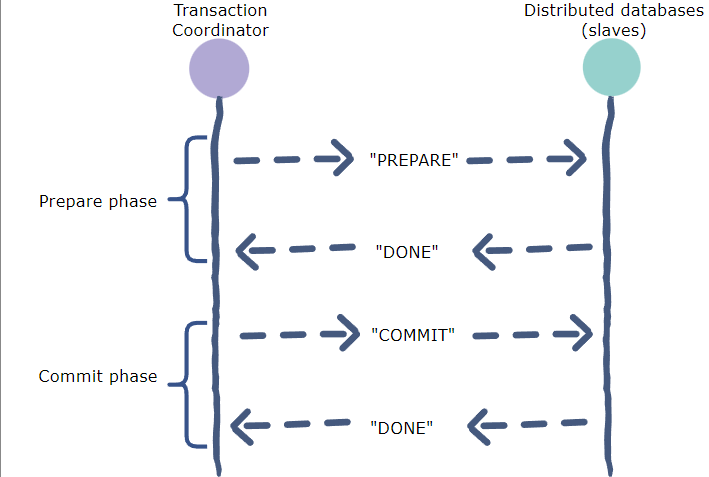
\includegraphics[width=8cm]{2pc.png}
\caption{Funcionamento do Protocolo 2PC}
\end{figure}

Para finalizar, o \ac{2PC}, está relacionado com os princípios já abordados anteriormente, \ac{ACID}, porque este protocolo garante a atomicidade, a consistência, o isolamento e a durabilidade de uma transação.


\section{Base de Dados Distribuídas}
Um sistema de bases de dados distribuídas consiste em múltiplos servidores, cada um responsável pelos seus dados. Estes dados podem ser acedidos utilizando uma rede e, apesar de estarem fisicamente distribuídos, devem apresentar-se ao utilizador logicamente integrados, como se estivessem num único servidor. 

\subsection{Divisão de Base de Dados Distribuídas}
Podemos dizer que Bases de Dados Distribuídas se encontram divididas em dois sistemas:

\begin{enumerate}
    \item Sistemas Homogéneos: todos os \textit{nodes}  usam o mesmo \ac{SGBD} mas os dados estão armazenados em várias \ac{BD}.
    \item Sistemas Heterogéneos: cada \textit{node} utiliza um \ac{SGBD} diferente onde partilham \ac{BD} pré existentes com mesmo modelo de dados ou modelos de dados diferentes. 
\end{enumerate}

\subsection{Vantagens e Desvantagens de Base de Dados Distribuídas}
\begin{itemize}
    \item Vantagens: Uma das vantagens para utilizar Base de Dados Distribuídas é pelo fato, como o nome indica, de ser de natureza distribuída. Ou seja, geograficamente se uma organização tiver várias sedes espalhadas pelo país faz sentido utilizar uma base de dados distribuída, pois vai espelhar a estrutura da organização, vai implicar que cada sede tenho o seu próprio servidor.
    Resumidamente, existe maior segurança, partilha de dados e autonomia local, desempenho melhorado (em relação ás \ac{BD}), fiabilidade/disponibilidade e é mais vantajoso para representar várias organizações.
    \item Desvantagem: Ao contrário da vantagem dada, não se justifica ter vários servidores espalhados quando uma organização possui geograficamente as suas delegações/sedes umas ao lado das outras. Neste caso faz mais sentido ter uma solução cliente/servidor.
    Resumidamente, tem custos de desenvolvimento de Software, maior possibilidade de erros no software, aumento da carga de processamento e aumento da complexidade da coordenação dos \textit{nodes}.
\end{itemize}

\cleardoublepage
\section{Sistema de Gestão de Base de Dados}
Um \ac{SGBD} é o software que gere o armazenamento, manipulação e pesquisa dos dados existentes na \ac{BD}, funcionando como uma interface entre as aplicações e os dados necessários para a execução dessas aplicações.\\*
\indent Exemplos \ac{SGBD}: Microsoft SQL Server, Oracle Server, MariaDB, MySQL, entre outros.


\begin{figure}[H]
\center
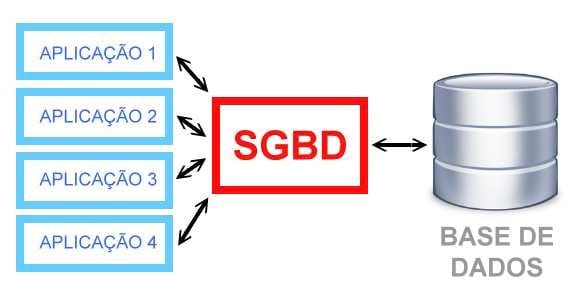
\includegraphics[width=8cm]{sgbd.jpg}
\caption{Arquitetura \ac{SGBD}}
\end{figure}

\subsection{Requisitos fundamentais de um SGBD}
\begin{itemize}
    \item Segurança: proteção da \ac{BD} contra acessos não autorizados;
    \item Integridade: validação de operações que coloquem em risco a consistência dos dados;
    \item Controlo de concorrência nos acessos: coordenação da partilha dos dados pelos vários utilizadores
    \item Recuperação de falhas: restaurar a integridade da \ac{BD} depois da ocorrência de uma falha. Mecanismos de recuperação (fundamentalmente baseados em redundância): backups, \textit{transaction logging} (ficheiro \textit{transaction log}, dados para repor as últimas transações).
\end{itemize}

\cleardoublepage
\section{Replicação de dados}
A replicação é a técnica de duplicar dados em vários \textit{nodes} diferentes. Para tornar a replicação segura existe um conjunto de razões para a duplicação dos dados, que passo a citar:

\begin{itemize}
    \item Prevenção contra falhas: a falha de um \textit{node} que contenha dados importantes ao sistema não compromete, necessariamente, o seu funcionamento;
    \item Redução da transferência de dados: há uma maior probabilidade de os dados estarem disponíveis localmente ou mais perto do \textit{node} que os requisita. Isto resulta na redução dos custos de transferência;
    \item Paralelismo: os pedidos à \ac{BD} podem ser processados por vários \textit{nodes} em paralelo, o que vai existir um maior desempenho.
\end{itemize}


Como não falamos só de vantagens, neste caso também existe desvantagens e neste cenário de replicação uma das desvantagens é a necessidade de manter uma coerência total do sistema. A coerência total do sistema implica que quando a informação num \textit{node} é atualizada, as suas réplicas também devem ser atualizadas, o que aumenta o \textit{overhead} do sistema (custos de atualização e necessidade de algoritmos complexos para a execução de transações).\\*
\indent Dentro do sistema, conforme as atualizações propagadas, a replicação pode ser \textbf{síncrona} (ocorre em tempo real e é preferida para sistemas com objetivos de baixo tempo de recuperação que não podem perder dados), \textbf{assíncrona} (replicação lenta e projetado para trabalhar em distâncias e requer menos largura de banda).\\*

Para concluir, quando os dados têm de estar permanentemente atualizados, é preferível recorrer à replicação síncrona. Caso contrário, deve-se utilizar a replicação assíncrona por ter melhores tempos de resposta e até é possível indicar intervalos de tempo para as atualizações.\\*

A replicação traz mais benefícios quando os dados são lidos muitas vezes pelos servidores remotos, mas poucas vezes atualizados, devido à carga adicional que é colocada sobre o sistema para manter as réplicas consistentes. 

\cleardoublepage

\section{Conclusão sobre o item (2) do enunciado}
O protocolo \ac{2PC} assegura que a propriedade da atomicidade da transação é respeitada. Caso exista um \textit{Abort} de um dos \textit{nodes} a transação falha.\\*
\indent O \ac{2PC} pode ficar inoperante devido à falha de um dos \textit{nodes} durante o processo. Uma transação inoperante não é desejável porque continua a manter os \textit{locks} dos recursos de que necessita para a sua transação, impedindo que outras transações que precisem desses mesmos recursos os possam obter.\\*
\indent O objetivo das técnicas de tolerâncias de falhas nas Base de Dados Distribuídas é garantir que não há perda/corrupção de dados.\\*
\indent O \ac{SGBD} é responsável por tudo, guardar os dados no disco rígido, manter em memória os dados mais acedidos, ligar dados e metadados (dados sobre outros dados), disponibilizar uma interface para programas e utilizadores. Isto são algumas das vantagens de um \ac{SGBD} mas como temos visto também tem as suas desvantagens. Trabalhar com três \ac{SGBD} implica utilizar mais do que um utilizador e não pode prejudicar nenhum deles. O controlo de acesso irá garantir a integridade dos dados com a possibilidade de configurar níveis de acesso a cada utilizador (segurança). 


\subsection{Falhas que podem ocorrer no 2PC}
\begin{itemize}
    \item Falhas nos \textit{nodes};
    \item Falhas na rede;
    \item Falhas de Software;
    \item Falha do coordenador.
\end{itemize}

\subsection{Desvantagens do 2PC}
Como já foi referido atrás, uma das desvantagens é o protocolo \ac{2PC} ser demasiado restritivo, basta que um dos \textit{nodes} falhe ou fique inoperável e os restantes \textit{nodes} efetuam um \textit{rollback}. Uma segunda desvantagem é se existir uma falha após a primeira fase (fase antes do envio das instruções de \textit{commit} ou \textit{abort}, todas as sub-transações ficam bloqueadas (num estafo de espera ativa mantendo os \textit{locks} que possuíam.

Para resolver estes problemas (Desvantagens acima descritas) foi criado o protocolo \ac{3PC}. Um protocolo não muito usado devido ao elevado tráfego que necessitava. O \ac{3PC} é um protocolo semelhante ao \ac{2PC} mas com um passo adicional intermédio \textit{Pre-Commit},que confirma se todos os \textit{nodes} estão em condições de finalização.
